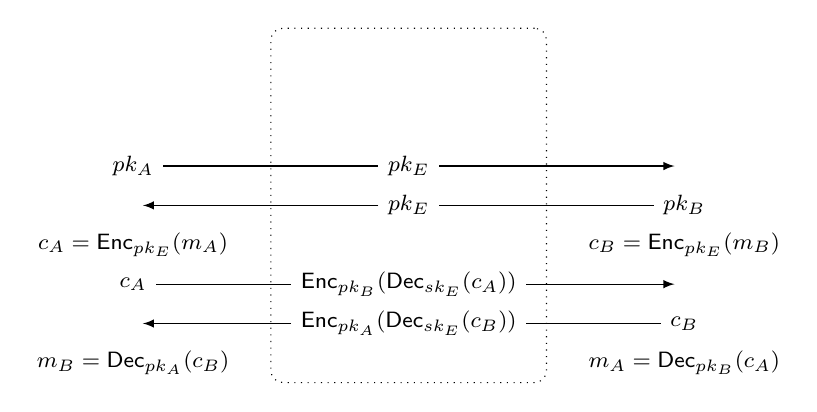
\begin{tikzpicture}[font=\footnotesize]
\node (A) at (0,0) {\Alice};
\node (E) [right of = A, node distance = 3.5cm] {\Adversary};
\node (B) [right of = E, node distance = 3.5cm] {\Bob};
\node (1a) [below of=A, node distance=1cm] {$pk_A$};
\node (1e) [below of=E, node distance=1cm] {$pk_E$};
\node (1b) [below of=B, node distance=1cm] {};
\draw[-latex] (1a) -- (1e) -- (1b) node [midway,above] {};
\node (2a) [below of=1a, node distance=0.5cm] {};
\node (2b) [below of=1b, node distance=0.5cm] {$pk_B$};
\node (2e) [below of=1e, node distance=0.5cm] {$pk_E$};
\draw[-latex] (2b) -- (2e) -- (2a) node [midway,above] {};
\node (4a) [below of=2a, node distance=0.5cm] {$c_A = \mathsf{Enc}_{pk_E}(m_A)$};
\node (4b) [below of=2b, node distance=0.5cm] {$c_B = \mathsf{Enc}_{pk_E}(m_B)$};
\node (4e) [below of=2e, node distance=0.5cm] {};
\node (5a) [below of=4a, node distance=0.5cm] {$c_{A}$};
\node (5b) [below of=4b, node distance=0.5cm] {};
\node (5e) [below of=4e, node distance=0.5cm] {$ \mathsf{Enc}_{pk_B}(\mathsf{Dec}_{sk_E}(c_A))$};
\draw[-latex] (5a) -- (5e) -- (5b) node [midway,above] {};
\node (6a) [below of=5a, node distance=0.5cm] {};
\node (6b) [below of=5b, node distance=0.5cm] {$c_{B}$};
\node (6e) [below of=5e, node distance=0.5cm] {$ \mathsf{Enc}_{pk_A}(\mathsf{Dec}_{sk_E}(c_B))$};
\draw[-latex] (6b) -- (6e) -- (6a) node [midway,above] {};
%\node (9a) [below of=6a, node distance=0.5cm] {$c_B = (c_{B1}\| c_{B2})$};
%\node (9b) [below of=6b, node distance=0.5cm] {$c_A = (c_{A1}\| c_{A2})$};
\node (10a) [below of=6a, node distance=0.5cm] {$m_B = \mathsf{Dec}_{pk_A}(c_B)$};
\node (10b) [below of=6b, node distance=0.5cm] {$m_A = \mathsf{Dec}_{pk_B}(c_A)$};
\node (11) at (3.5cm,-1.5cm) [minimum height=4.5cm, minimum width=3.5cm, dotted, draw,rounded corners=1ex] {};
\end{tikzpicture}
